\documentclass{article}
\usepackage[utf8]{inputenc}
\usepackage[T2A]{fontenc}
\usepackage[utf8]{inputenc}
\usepackage[russian]{babel}
\usepackage[margin=3cm]{geometry}
\usepackage{paralist}
\usepackage{amsthm, amsmath, amsfonts, amssymb}
\usepackage{mathtools} % \mathclap
\usepackage{bm}
\usepackage{dsfont}
\usepackage{hyperref}
\usepackage{graphicx}
\usepackage{multirow}
\usepackage{comment}
\usepackage{xcolor, colortbl}
\usepackage{xifthen, xspace}
\usepackage{caption, subcaption}
\usepackage{lscape}
\usepackage{braket}
\usepackage{epigraph}
\usepackage{sectsty}
\usepackage{listings}
\usepackage{graphicx}

\hypersetup{
    colorlinks=true,
    linkcolor=blue,
    filecolor=magenta,      
    urlcolor=blue,
    pdftitle={Overleaf Example},
    pdfpagemode=FullScreen,
    }

\title{Теоретические модели вычислений \\
ДЗ №3: Машины Тьюринга и квантовые вычисления}

\date{1 мая 2022 года}

\begin{document}
\begin{center}
"Теоретические модели вычислений ДЗ№3" \\
Бородин Сергей Владимирович А-13а-19
\end{center}
\vspace{6em}




\newpage

\maketitle

\section{Машины Тьюринга}

Работу требуется выполнять в системе \url{turingmachine.io}. \\\\
Для сдачи заданий 1-2 требуется прикрепить файлы YAML с исходным кодом проекта. Каждый файлы должен иметь наименование задание\_пункт.yml, к примеру 1\_1.yml для первой задачи первого задания. \\\\

\subsection{Операции с числами}

Реализуйте машины Тьюринга, которые позволяют выполнять следующие операции:
\begin{enumerate}
    \item Сложение двух унарных чисел (1 балла)\\\\
    \text(Алгоритм: Машина Тьюринга принимает строку состоящую из двух унарных чисел разделенных +. Машина будет 
    переносить посимвольно первое число в конец второго числа, а в конце когда в начеле будет + затрет его и закончит работу. Исходный код лежит в файле 1-1. yaml) 
    \item Умножение унарных чисел (1 балл)\\\\
    \text(Алгоритм: Машина Тьюринга принимает строку состоящую из двух унарных чисел разделенных *. Машина будет затирать один символ первого числа, а затем копировать все единицы второго числа в после второго числа, этот процесс будет повторятся пока первое число не затрется. После Машина затрет второе число и знак * и завершит работу. Исходный код лежит в файле 1-2. yaml)
\end{enumerate}


\subsection{Операции с языками и символами}

Реализуйте машины Тьюринга, которые позволяют выполнять следующие операции:
\begin{enumerate}
    \item Принадлежность к языку $L = \{ 0^n1^n2^n \}, n \ge 0$ (0.5 балла)\\\\
    \text(Алгоритм: Машина Тьюринга принимает строку состоящую из 0 1 2. Машина будет искать 0, превращать его в *, возврпщаться в начало после искать 1 и возвращаться в начало, после искать 2 и возвращатьсся в начало. В случае, если при поиске 0 будет найден ' ', то проверяется, что все предыдущие элементы строки *, и в этом случае выводится 'Т'. В случае, если ' ' найден в случае поиска 1 или 2, то выводится 'F', так же онео выводится, если при проверке строки на '*', найдет какой-то другой элемент, то в конце тоже выводится 'F'. После вывода 'Т' или 'F', машмна завершаеет работу. Исходный код лежит в файле 2-1. yaml)\\\\
    \item Проверка соблюдения правильности скобок в строке (минимум 3 вида скобок) (0.5 балла)
    \text(Алгоритм: Машина Тьюринга принимает строку состоящую из ( { [ ) ] }. Машина будет искать закрывающую скобку и менять ее на символ, потом идти налево и искать соответствующею открывающую ее тоже менять на символ, при этом, если будет находить ошибочно открытая, то ставить N и затирать все кроме нее. Процесс будет повторяться, пока уйдут все скобки, либо не выявется ошибка. Исходный код лежит в файле 2-2-1. yaml)
    \item Поиск минимального по длине слова в строке (слова состоят из символов 1 и 0 и разделены пробелом) (1 балл)\\\\
    \text(Алгоритм: Машина Тьюринга принимает строку состоящую из 1 0 ' '. Машина будет искать Машина будет идти до конца строки и ставит флажок, далее возвращать нязад и идти по каждому слову и менять на первую букву слова на символ, потом процесс повторится для вторых букв и так далее, в итоге, когда вместо буквы будет найден ' ', слово будет "помечено", а остальные слова затеры, полученное слово приведется в нормальный вид. Исходный код лежит в файле 2-3. yaml)
\end{enumerate}


\section{Квантовые вычисления}

Для выполнения заданий по квантовым вычислениям требуется QDK. Его можно скачать здесь: \url{https://docs.microsoft.com/en-us/azure/quantum/install-overview-qdk}. 
\\\\
Но можно использовать любой пакет, типа \url{https://qiskit.org/}. 
\\\\
В качестве решения задачи надо предоставить схему алгоритма для частного случая при фиксированном количестве кубитов и фиксированных состояниях. 


\subsection{Генерация суперпозиций 1 (1 балл)}

Дано $N$ кубитов ($1 \le N \le 8$) в нулевом состоянии $\Ket{0\dots0}$. Также дана некоторая последовательность битов, которое задаёт ненулевое базисное состояние размера $N$. Задача получить суперпозицию нулевого состояния и заданного.

$$\Ket{S} = \frac{1}{\sqrt2}(\Ket{0\dots0} +\Ket{\psi})$$

То есть требуется реализовать операцию, которая принимает на вход:

\begin{enumerate}
    \item Массив кубитов $q_s$
    \item Массив битов $bits$ описывающих некоторое состояние $\Ket{\psi}$. Это массив имеет тот же самый размер, что и $qs$. Первый элемент этого массива равен $1$.
\end{enumerate}


\begin{lstlisting}
operation Solve (qs: Qubit[], bits: Bool[]) : () 
{
    body 
    {
        H(qs[0]);  
        for (i in 1..Length(qs) - 1)
        {

            if (bits[i]) 
            {
                CNOT(qs[0], qs[i]);
            }
        }
    }
}




\end{lstlisting}
\text{Для входный данных |0 0 0 0⟩,  |1 0 1 0⟩ схема алгоритма будет выглядеть следующим образом:}\\
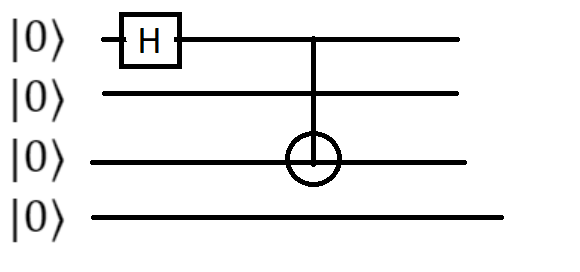
\includegraphics [scale=0.5]{3_1.png}\\\\\

\subsection{Различение состояний 1 (1 балл)}

Дано $N$ кубитов ($1 \le N \le 8$), которые могут быть в одном из двух состояний:

$$\Ket{GHZ} = \frac{1}{\sqrt2}(\Ket{0\dots0} +\Ket{1\dots1})$$
$$\Ket{W} = \frac{1}{\sqrt N}(\Ket{10\dots00}+\Ket{01\dots00} + \dots +\Ket{00\dots01})$$

Требуется выполнить необходимые преобразования, чтобы точно различить эти два состояния. Возвращать $0$, если первое состояние и 1, если второе. 
\\\\
\begin{lstlisting}
operation Solve (qs: Qubit[]) : Int
{
    body 
    {
        mutable countOnes = 0;
        for (i in 0..Length(qs) - 1)
        {
            if (M(qs[i]) == One)
            {
                set counter = counter + 1;
            }
        }
        if (counter == 1)
        {
            return 1;
        }
        return 0;
    }
}

\end{lstlisting}


\subsection{Различение состояний 2 (2 балла)}

Дано $2$ кубита, которые могут быть в одном из двух состояний:

$$\Ket{S_0} = \frac{1}{2}(\Ket{00} + \Ket{01} + \Ket{10} + \Ket{11})$$
$$\Ket{S_1} = \frac{1}{2}(\Ket{00} - \Ket{01} + \Ket{10} - \Ket{11})$$
$$\Ket{S_2} = \frac{1}{2}(\Ket{00} + \Ket{01} - \Ket{10} - \Ket{11})$$
$$\Ket{S_3} = \frac{1}{2}(\Ket{00} - \Ket{01} - \Ket{10} + \Ket{11})$$


Требуется выполнить необходимые преобразования, чтобы точно различить эти четыре состояния. Возвращать требуется индекс состояния (от $0$ до $3$). 
\\\\
\begin{lstlisting}
operation Solve (qs: Qubit[]) : Int
    {
        body 
        {
			H(qs[0]);
			H(qs[1]);
			if (M(qs[0]) == Zero) 
			{
				if (M(qs[1]) == Zero)
				{
					return 0;
				}
				else
				{
					return 1;
				}
			}
			else
			{
				if (M(qs[1]) == Zero)
				{
					return 2;
				}
				else
				{
					return 3;
				}
			}
        }
    }

\end{lstlisting}


\subsection{Написание оракула 1 (2 балла)}

Требуется реализовать квантовый оракул на $N$ кубитах ($1 \le N \le 8$), который реализует следующую функцию: $f(\pmb{x}) = (\pmb{b}\pmb{x}) \mod 2$, где  $\pmb{b} \in \{0,1\}^N$ вектор битов и  $\pmb{x}$ вектор кубитов. Выход функции записать в кубит $\pmb{y}$. Количество кубитов $N$ ($1 \le N \le 8$). 
\\\\
Заготовка для кода:
\begin{lstlisting}
namespace Solution {
        open Microsoft.Quantum.Primitive;
        open Microsoft.Quantum.Canon;
        operation Solve (x : Qubit[], y : Qubit, b : Int[]) : ()
        {
            body
            {

            }
        }
}
\end{lstlisting}

\end{document}